
\section{MLP based model Evaluation}\label{sec:mlpeval}
From the training phase graph shown in Figure~\ref{fig:ufcntraining},
we can see that it has concluded successfully because the two curves
(training loss and validation loss) do not diverge but remain at a
relatively constant distance from each other.
This also suggests that there is no overfitting.
However, the values of the two loss functions do not appear to decrease
significantly as the epochs progress, indicating that the model may
not have generalized well.


%Dal grafico della fase di training mostrato in Figura~\ref{fig:ufcntraining}
%possiamo evicnere come questa sia terminata con successo dal
%fatto che le due curve (training loss e validation loss) non divergono
%ma rimangono ad una distanza abbastanza costante e possiamo
%anche capire che non ci sia presenza di overfitting.
%I valori delle due loss però non sembrano scendere col passare
%delle epoche ma rimangono pressochè costanti, indice che il modello
%potrebbe non essere riuscito a generalizzare bene.

From the graphs in Figure~\ref{fig:ufcnsysusage}, it is apparent that the
machine on which this model was trained was relatively underutilized.
In particular, it's worth noting that GPU utilization did not exceed 30\%,
and GPU memory was barely utilized, staying at around 20\%.
This suggests that the model can be trained on less powerful machines as well.
The model is also relatively lightweight in terms of memory,
with just 100 MB (see Table~\ref{tab:ufcnspecs}), and the training time
did not exceed 30 seconds.
Inference time is extremely fast, taking less than a second.

%Dai grafici in Figura~\ref{fig:ufcnsysusage} possiamo notare come
%la macchina su cui è stato addestrato questo modello sia stata
%sfruttata relativamente poco, in particolare facciamo notare come
%l'utilizzo della GPU non ha superato il 30\% e la sua memoria è stata
%a malapena occupata per il 20\%. Questo può portarci ad affermare che
%il modello può essere anche addestrato su macchine molto meno performanti
%della nostra. Il modello risulta essere anche relativamente leggero sia
%in termini di memoria, soli 100 MB (vedi Tabella~\ref{tab:ufcnspecs}) sia
%per il tempo di allenamento che non ha superato i 30 secondi. Il tempo di
%inferenza risulta estremamente veloce non superando il secondo.


\begin{table}[H]
	\begin{center}
		\begin{tabular}[c]{l|l|l|l}
			%\cline{2-4}
			\multicolumn{1}{c|}{\textbf{Gap period}} &
			\makecell{\textbf{MAE} \textbf{(kW)}}    &
			\makecell{\textbf{MAPE} \textbf{(\%)}}   &
			\multicolumn{1}{c}{\textbf{R}$^2$}                               \\
			\hline
			02-04 to 03-04                           & 18.63 & 128.47 & 0.64 \\
			03-04 to 04-04                           & 06.90 & 64.97  & 0.52 \\
			05-04 to 06-04                           & 17.99 & 109.78 & 0.42 \\
			06-04 to 07-04                           & 20.07 & 113.99 & 0.62 \\
			11-04 to 12-04                           & 10.66 & 33.84  & 0.92
		\end{tabular}
	\end{center}
	\caption{The table displays the values of MAE (Mean Absolute Error)\cite{metrics}, MAPE (Mean Absolute Percentage Error)\cite{metrics} and the R$^2$ (R-squared)\cite{metrics} index applied to the model predictions shown in Figures~\ref{fig:ufcnevalbelli} and \ref{fig:ufcnevalbrutti}.}\label{tab:ufcnndatitab1}
	%La tabella mostra i valori del MAE e dell'indice R$^2$ applicate alle predizioni del modello mostrate nelle Figure~\ref{fig:ufcnevalbelli} e \ref{fig:ufcnevalbrutti}.}\label{tab:dfsplit}
\end{table}

\begin{table}[H]
	\centering
	\begin{tabular}{l|l|l|l}
		                                        &
		\multicolumn{1}{c|}{\textbf{MAE (kW)}}  &
		\multicolumn{1}{c|}{\textbf{MAPE (\%)}} &
		\multicolumn{1}{c}{\textbf{R$^2$}}                             \\
		\hline
		\textbf{AVG}                            & 14.11 & 70.98 & 0.69 \\
		\textbf{STD. DEV}                       & 3.81  & 27.99 & 0.17
	\end{tabular}
	\caption{MLP based model Global metrics.}
	\label{tab:globalmetrics}
\end{table}
%\begin{table}[H]
%	\begin{center}
%		\begin{tabular}[c]{l|l|l|c|c|c|c}
%			%\cline{2-4}
%            \multicolumn{1}{c|}{\textbf{Gap}}& 
%            \makecell{\textbf{MAE}\\\textbf{(kW)}} &
%            \multicolumn{1}{c|}{\textbf{R}$^2$} &
%            \multicolumn{2}{c|}{\textbf{Day 1}} &
%            \multicolumn{2}{c}{\textbf{Day 2}} \\
%			\hline
%
%         %& & & \tiny \textbf{MAE (kW)} & \tiny \textbf{MAPE (\%)} & \tiny \textbf{MAE (kW)} & \tiny \textbf{MAPE (\%)}\\
%         & & & \small \makecell{\textbf{MAE}\\\textbf{(kW)}} & \small \makecell{\textbf{MAPE}\\\textbf{(\%)}} & \small \makecell{\textbf{MAE}\\\textbf{(kW)}} & \small \makecell{\textbf{MAPE}\\\textbf{(\%)}}\\
%         \cline{4-7}
%           02-04 to 03-04 & 18.63 & 0.64 &1774.87&36.32&1774.87&199.20 \\
%           03-04 to 04-04 & 06.90 & 0.52 &355.04&39.85&355.04&24.35 \\
%           05-04 to 06-04 & 17.99 & 0.42 &152.34&7.23&152.34&5.97 \\
%           06-04 to 07-04 & 20.07 & 0.62 &1293.53&50.70&1293.53&25.22 \\
%		\end{tabular}
%	\end{center}
%	\caption{The table displays the values of MAE (Mean Absolute Error)\cite{metrics} and the R$^2$ (R-squared)\cite{metrics} index applied to the model predictions shown in Figures~\ref{fig:ufcnevalbelli} and \ref{fig:ufcnevalbrutti}.}\label{tab:grrundatitab1}
% %La tabella mostra i valori del MAE e dell'indice R$^2$ applicate alle predizioni del modello mostrate nelle Figure~\ref{fig:ufcnevalbelli} e \ref{fig:ufcnevalbrutti}.}\label{tab:dfsplit}
%\end{table}
%
\begin{figure}[H]
	\centering
	\begin{subfigure}{\textwidth}
		\centering
		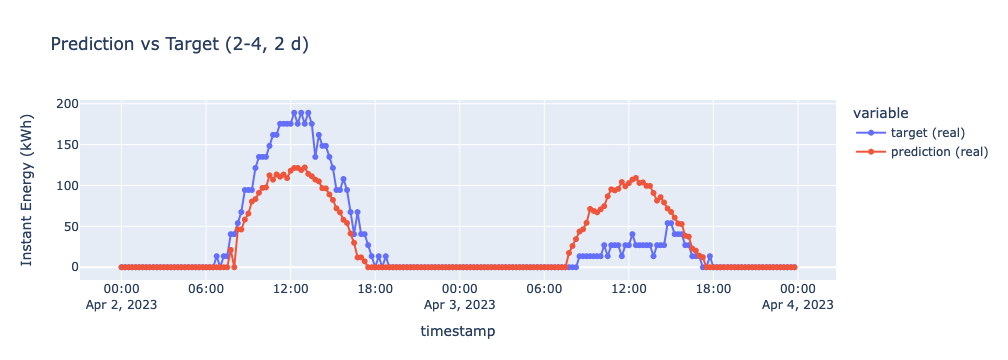
\includegraphics[width=.8\textwidth]{chapters/3_models/imgs/ufnc/eval/ufcpred2-4.png}
		\caption{}
	\end{subfigure}
	\begin{subfigure}{\textwidth}
		\centering
		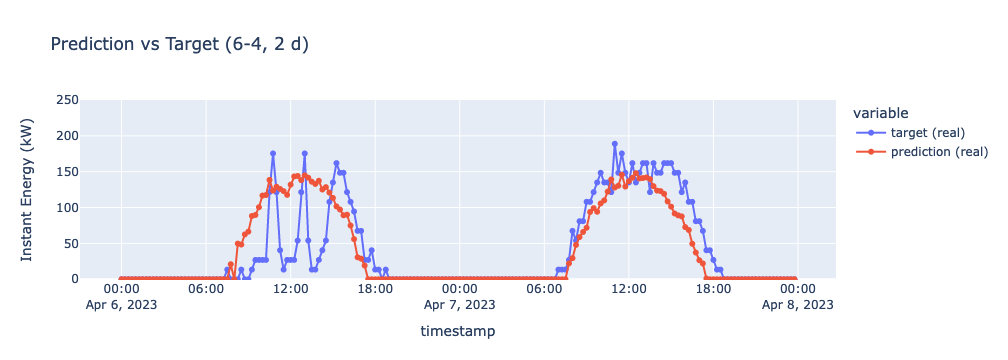
\includegraphics[width=.8\textwidth]{chapters/3_models/imgs/ufnc/eval/ufcpred6-4.png}
		\caption{}
	\end{subfigure}
	\begin{subfigure}{\textwidth}
		\centering
		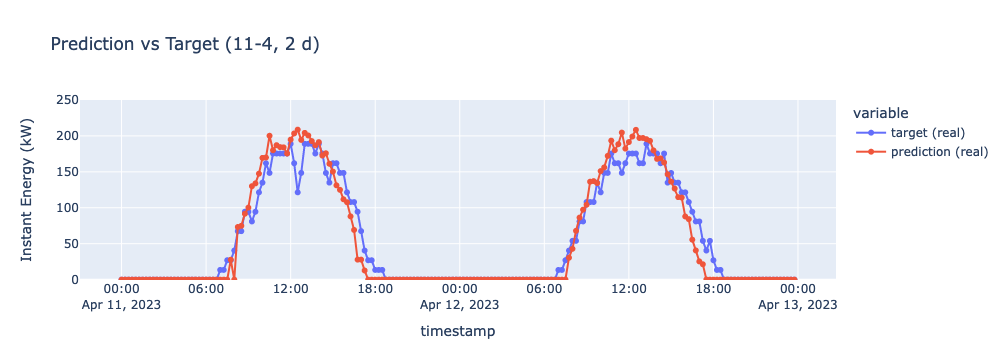
\includegraphics[width=.8\textwidth]{chapters/3_models/imgs/ufnc/eval/ufcpred11-4.png}
		\caption{}
	\end{subfigure}
	\caption{The figure displays three predictions made by the model, where you can observe the network's output (in red) and the ground truth (in blue). The model was tested on two gaps, each covering a period of 2 days. The first gap (a) spans from 02-04-2023 to 04-04-2023, the second gap (b) spans from 06-04-2023 to 06-08-2023
		and the third starts from 11-04-2023 to 12-04-2023.}

	%La figura riporta due predizioni del modello dove possiamo apprezzare l'output della rete (in rosso) e la ground trought (in blu). Al modello sono stati fatti chiudere due buchi di 2 giorni ciuascuno che coprono rispettivamente il periodo dal 02-04-2023 al 04-04-2023 e dal 06-04-2023 al 06-08-2023.}
	\label{fig:ufcnevalbelli}
\end{figure}

Analyzing the graphs presented in Figure~\ref{fig:ufcnevalbelli},
we can confirm the previous suspicion that the model did not learn well how
to predict the trend of instant energy production from the plant.
Plot (a) clearly illustrates how the model's prediction is very timid
and fails to grasp the possibility that some days may be more productive
than others.
In graph (b), we can see how the model almost approximates the second
day but makes a significant mistake on the first,
failing to understand the potential for production spikes during the day. In (c), on the other hand, we can see
how the model's output manages to understand the
ground truth's behavior quite well. In fact,
we have an $R^2$ index value of 0.96 and low values for MAE and MAPE. These claims are supported by the data shown in Table~\ref{tab:ufcnndatitab1}.

It's also evident that the model struggles to handle the
day/night cycle, often ending production much earlier than it should.
However, it consistently predicts zero energy production
during the night, which is a positive aspect.

%Analizzando i grafici mostrati in Figura~\ref{fig:ufcnevalbelli} possiamo
%confermare il sospetto precedente, il modello non è riuscito ad apprendere
%bene come predirre l'andamento della curva dell'energia istantanea prodotta
%dall'impianto. Il plot (a) mostra molto bene come la predizione del modello sia
%molto timida e non riesce minimamente a comprendere la possibilità che alcuni
%giorni possono essere più produttivi di altri. Mentre nel grafico (b) possiamo
%vedere come il modello riesce quasi ad approssimare il secondo giorno, ma sbagliando
%notevolmente nel primo non risucendo a comprendere la possibilità di picchi di produzione durante la giornata.
%In (c) invece possiamo vedere come 
%l'output del modello riesce a comprendere abbastanza
%bene l'andamento della ground turth, infatti abbiamo 0.96
%come valore dell'indice $R^2$ e dei relativi valori bassi
%per MAE e MAEP. Le precedenti affermazioni sono motivate
%dai dati mostrati nella Tabella~\ref{ufcnndatitab1}.
%Si evince inoltre come questo ha difficoltà nel gestire il ciclo giorno/notte
%dato che molto spesso fa terminare la produzione molto prima di quando dovrebbe.
%Ottimo però il fatto che la produzione notturna risulti sempre nulla.

\begin{figure}[H]
	\centering
	\begin{subfigure}{\textwidth}
		\centering
		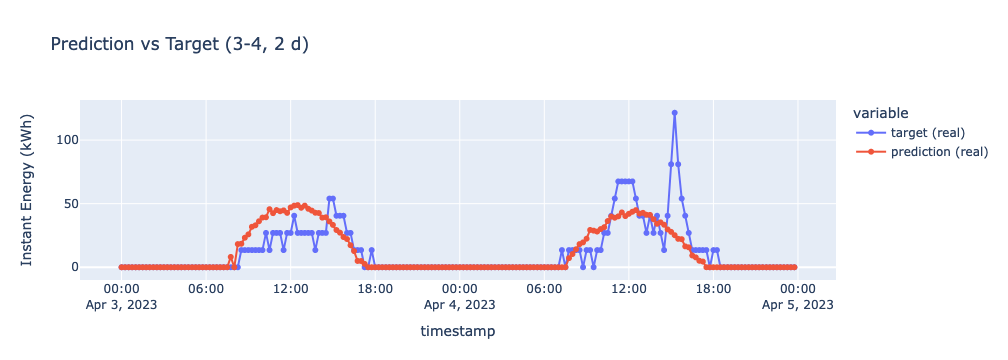
\includegraphics[width=.8\textwidth]{chapters/3_models/imgs/ufnc/eval/ufcpred3-4.png}
		\caption{}
	\end{subfigure}\\
	\begin{subfigure}{\textwidth}
		\centering
		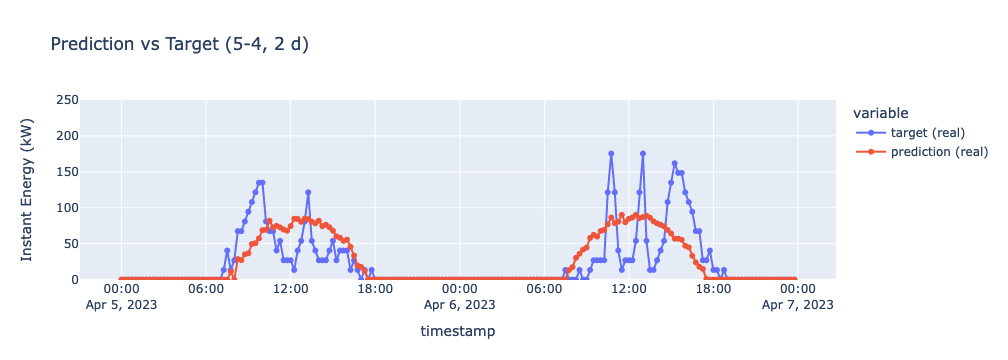
\includegraphics[width=.8\textwidth]{chapters/3_models/imgs/ufnc/eval/ufcpred5-4.png}
		\caption{}
	\end{subfigure}
	\caption{The figure displays two model predictions (in red) for two-day gaps and their respective ground truth (in blue). (a) corresponds to a gap from 03-04-2023 to 04-04-2023, while (b) covers the period from 05-04-2023 to 06-04-2023.}
	%In figura sono mostrati due predizioni del modello (in rosso) relative a buchi di due giorni e le rispettive ground truth (in blu). (a) fa riferimento ad un buco che va dal 03-04-2023 fino al 04-04-2023, mentre (b) copre il periodo che va dal 05-04-2023 fino al 06-04-2023.}
	\label{fig:ufcnevalbrutti}
\end{figure}

Figure~\ref{fig:ufcnevalbrutti} highlights the significant limitations
of the model, demonstrating how it fails to identify potential peak
values in production and how the predicted day curves are consistently similar
to each other.
It's also important to note that the model can only work with
gaps of a fixed size, and if a gap of a larger size is encountered,
it would be necessary to retrain the model.

%La Figura~\ref{fig:ufcnevalbrutti} mette in risalto i notevoli limiti del modello
%mostrando come non riesca minimamente ad individuare possibili valori di picco della 
%produzione e come le curve dei giorni predetti siano sempre molto simili tra di loro.
%\'{E} anche opportuno segnalare il fatto che il modello possa solo lavorare con
%buchi di dimensione sempre fissa e, qualora si presentasse un buco di più gradi 
%dimensioni sia necessario dover riallenare nuovamente il modello.


Analyzing the data presented in Tables~\ref{tab:ufcnndatitab1}
and \ref{tab:globalmetrics}, it can be confirmed that the performance
of this model is quite limited.
The $R^2$ index hovers around 0.60, with an average of 0.69 and a standard deviation of 0.17. This indicates that the target curve is not well approximated by the model's output.
While the \textit{MAE} appears to be relatively low (it's
important to consider that the nighttime period significantly lowers
the average, as the difference between target and prediction is zero during that time) the values of \textit{MAPE} are quite high, at times even reaching 100\% error, with an average value of 71\% and a standard deviation of 28\%.

In conclusion, despite the presented model being relatively
straightforward to implement and train, it is not suitable for
effectively addressing the problem of imputation.

%Analizzando anche i dati riportati nelle Tabelle~\ref{tab:grrundatitab1} e \ref{tab:globalmetrics} possiamo confermare che le prestazioni di questo
%modello sono abbastanza scarse. L'indice $R^2$ è quasi sempre inferiore a 
%0.6 il che vuol dire che la curva target non è stata bene approssimata
%dall'output del modello. Seppure il \textit{Gap MAE} risulti abbastanza basso, è da
%considerarsi che il periodo notturo tende ad abbassare nettamente la media
%in quanto la differenza tra target e prediction è nulla, i valori dei Daily MAE e MAPE risultano molto elevati, raggiungendo alcune volte anche il 200\% di errore. Possiamo concludere che, nonstante il modello presentato sia
%di semplice implementazione e addestramento
%risulti
%non essere adeguato per assolver al compito di risolvere il problema dell'Imputation.